\begin{table}[htbp]
	\centering
	\caption{List of measurement equipment and components}\label{tab_appendix:LaSetUp}
	
	\begin{tabularx}{\textwidth}{lXXXX}
		Name 				& Brand	& Model & AAU-number									\\ \toprule \rowcolor{lightGrey}
		
		DC motor & Alsthom BBC & F9M2 & 08339 
	\end{tabularx}
\end{table}


\subsubsection*{Setup}
\autoref{fig:KeMeasurementSetup} shows a diagram and photo of the measurement set up
\begin{figure}[htbp]
	\centering
	\begin{subfigure}{0.50\textwidth}
		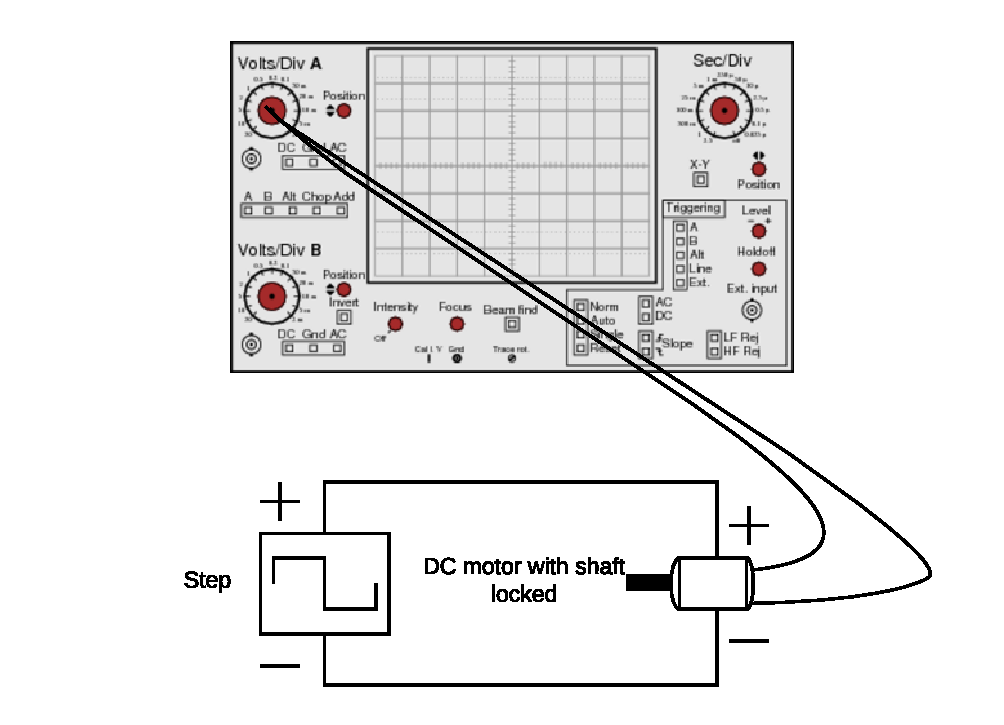
\includegraphics[width=\textwidth]{figures/appendix/Motor&GearTests/RmLmDiagram}
		\caption{Diagram of the setup.} \label{fig:RmLmMeasurementDiagram}
	\end{subfigure}
	\begin{subfigure}{0.40\textwidth}
		%\includegraphics[width=1\textwidth]{MotorImpedanceTest.jpg}
		\missingfigure{Picture of the setup}
		\caption{Picture of the setup.} \label{fig:RmLmMeasurementPictures}
	\end{subfigure}
	\caption{The measurement setup.} \label{fig:RmLmMeasurementSetup}   
\end{figure}

\subsubsection*{Method}
The test will consist of applying a step of \SI{7}{\volt} on the DC motor (which is at \SI{0}{\volt} before that) with its shaft locked. Then via a curve fitting tool named SENSETOOL $R_m$ and $L_m$ are deduced.

\subsubsection*{Raw Data}

\begin{figure}[htbp]
	\centering
	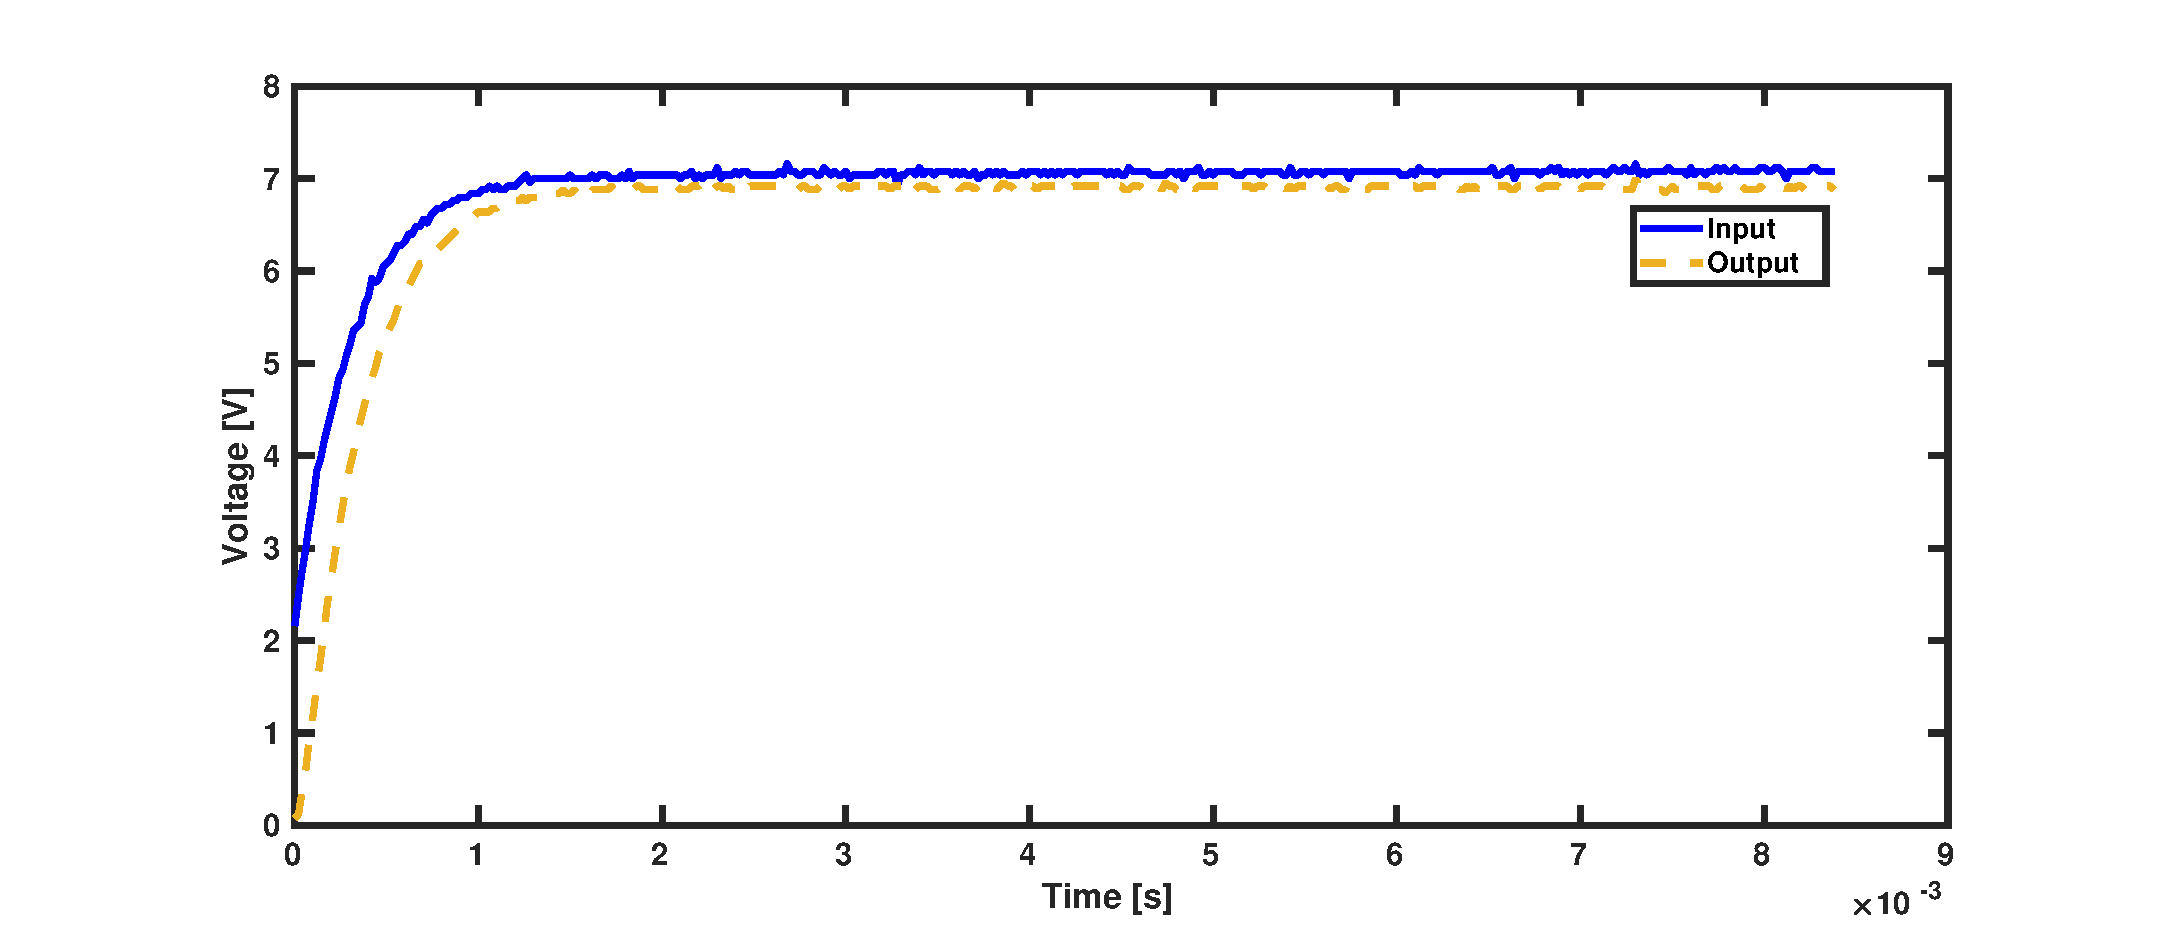
\includegraphics[width=\textwidth]{figures/appendix/Motor&GearTests/RmLmDataPlot}
	\caption{Plot of the voltage in respect to time of the input and the output of the DC motor}\label{fig:RmLmTestDataPlot}
\end{figure}

\subsubsection*{Data processing}

Since the shaft is locked, a step is applied and only the electrical characteristics of the motor are looked at. The data measured follows \autoref{eq:RmLmChar}.

\begin{equation}\label{eq:RmLmChar}
	u(t)=R_m i(t)+L_m \frac{\partial i(t)}{\partial t} \addunit{\volt}
\end{equation}

Which gives the transfer function \autoref{eq:RmLmTf}. Which is used to find $R_m$ and $L_m$ by curve fitting.

\begin{equation}\label{eq:RmLmTf}
\frac{I(s)}{U(s)}=\frac{1}{R_m +L_m s} \addunit{1}
\end{equation}

\subsubsection*{Conclusion}

After the curve fitting the following values are found $R_m=\SI{1.02}{\ohm}$ and $L_m=\SI{142}{\micro\henry}$. \autoref{fig:RmLmTestFitPlot} is a comparison between the model with these parameters and the measures done.

\begin{figure}[htbp]
	\centering
	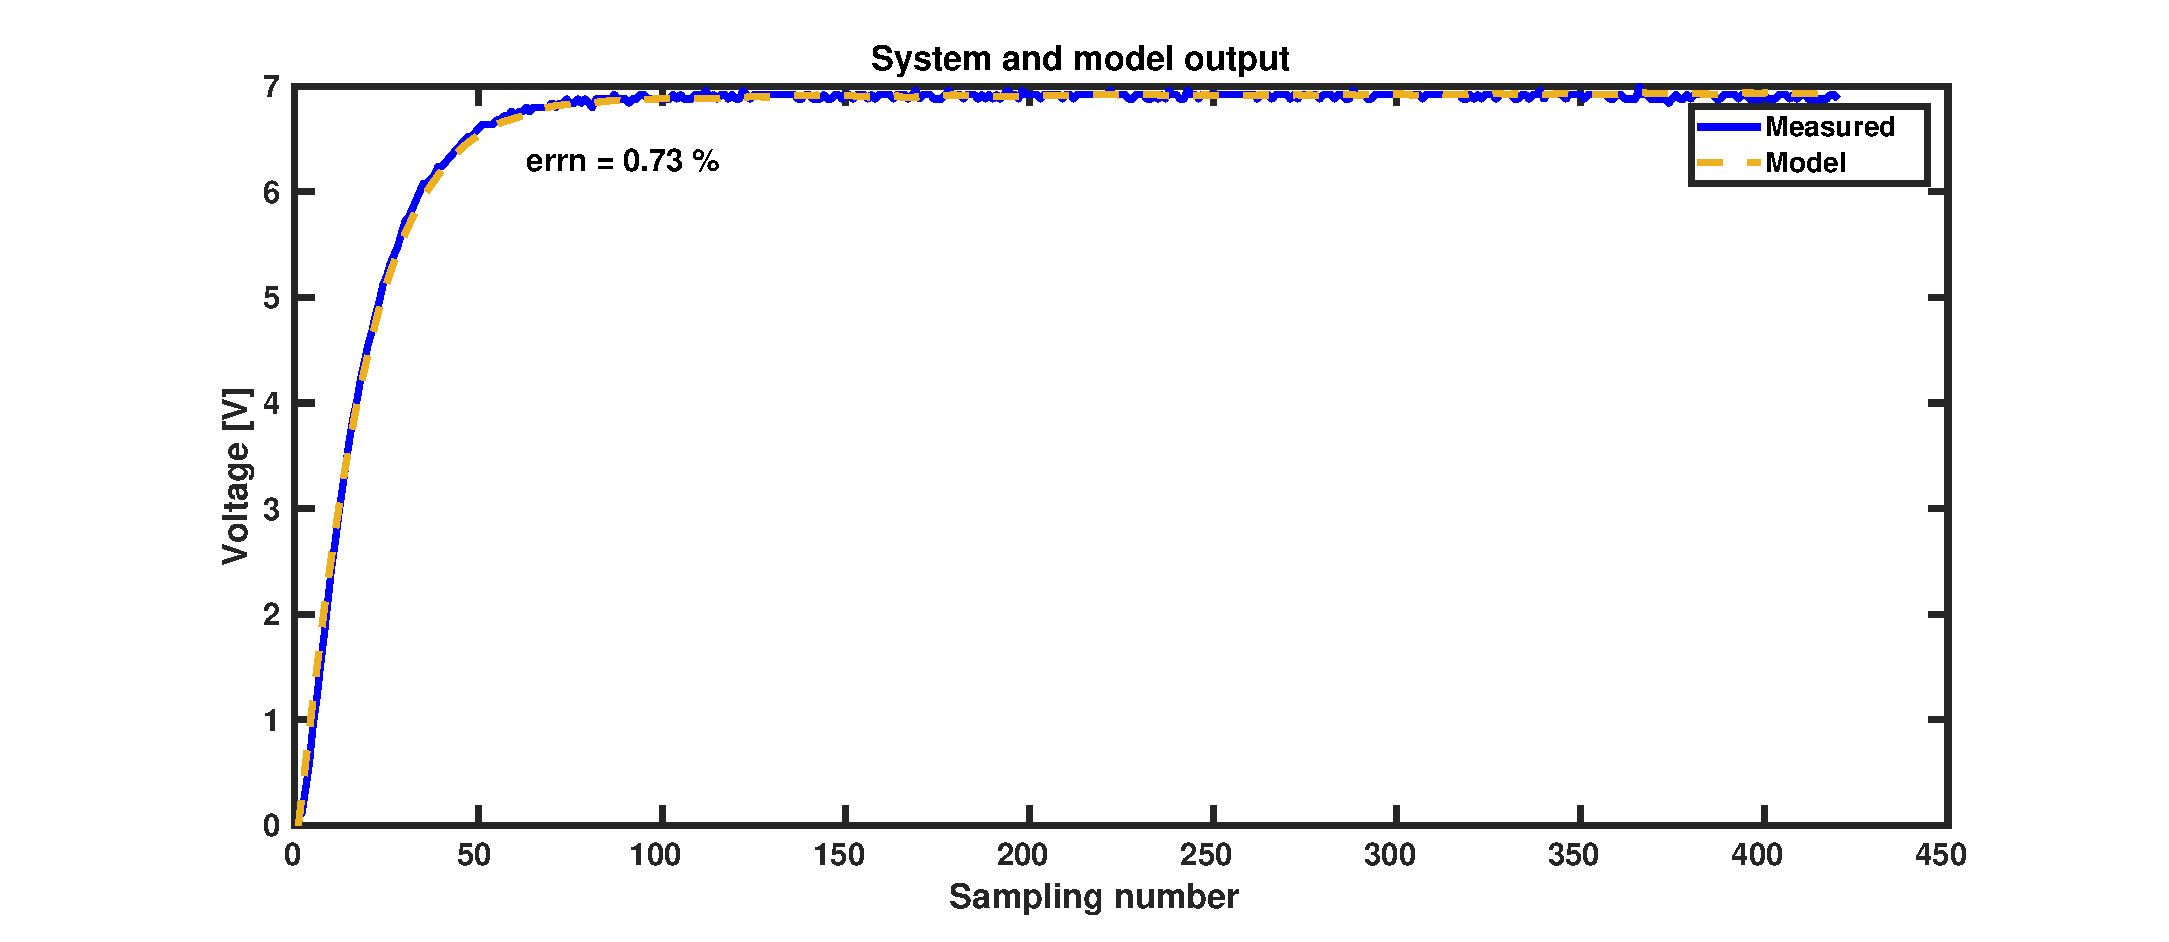
\includegraphics[width=\textwidth]{figures/appendix/Motor&GearTests/RmLmFitPlot}
	\caption{Plot of the comparison between the model and the measures}\label{fig:RmLmTestFitPlot}
\end{figure}
